\subsection{Genetic Algorithm Approach}
\label{sec:genetic_algorithm_optimisation}
% Point heavily to SPEA2 paper etc.
% Just want to give an overview of how these things work
% Fitness, Mating, Strength etc. -> what happens?
% define feasible, non-dominated, individual, generation etc.
In a genetic algorithm, a set of individuals -- a single point in multi-dimensional parameter space -- known as a population are randomly generated in the bounded parameter space; all of these points are feasible solutions to the optimisation problem. The objective functions are then calculated for each individual based on these variables and a fitness function, dependent on the objective functions, that measures how well an individual meets the optimization goals \cite{hofler2013innovative} is then evaluated. The design of fitness functions vary greatly between different genetic algorithms. The individuals are then evaluated against each other via a competition -- typically a head-to-head fitness comparison between pairs of individuals -- where the fitter (higher fitness) individuals that triumph over other individuals are selected to form a subset named the mating pool. The mating pool is the set of individuals which dominate (triumph over) other individuals in the population and aren't dominated by any other individual -- they are non-dominated. The mating pool individuals are the subset of the population which will form the next generation, which is the new population of the next iteration. In most GA's some non-dominated points of the previous generation are also inducted into the next generation. Individuals in the mating pool are paired together (randomly or otherwise) and through recombination, the exchange of variable values, and mutation, adjustment (scaling) of single parameter space variables \cite{hofler2013innovative} -- designed to mimic biological reproduction -- a set of new individuals for the next generation, named offspring, are produced.

Therefore, a genetic algorithm operates with a general basic procedure to solve a multi-dimensional multi-objective optimisation problem:
\begin{enumerate}
    \item{A population of individuals are randomly generated to sample the parameter space.}
    \item{Objective and fitness functions are evaluated for each individual in the new generation}
    \item{All non-dominated individuals of the previous generation are introduced (step doesn't apply in generation 1). }
    \item{If a termination condition is met, for example the no. generations exceeds a pre-set value, the simulation stops and the non-dominated individuals make up the Pareto front. }
    \item{A form of competition is used to select candidates to form the mating pool, which decides the composition of individuals in the next generation.}
    \item{Individuals in the mating pool are paired together (randomly or otherwise) and these produce the individuals of the next generation via recombination and mutation}
    \item{A new generation begins. The simulation is iterated starting from step 2. This repeats until the termination condition in step 4 is satisfied.}
\end{enumerate}
Once the termination condition has been satisfied, the Pareto-optimal front is produced and the parameters of all of the non-dominated individuals that constructed the Pareto-optimal front are returned. 

The genetic algorithm (GA) optimisation uses the minimisation routine of \textsc{SPEA2} \cite{zitzler2001spea2} within the \textsc{PISA} platform \cite{bleuler2003pisa} framework, following the methodology outlined by A. Hofler et al \cite{hofler2013innovative}. The \textsc{SPEA2} algorithm is a multi-objective evolutionary algorithm which incorporates a fine grained fitness assignment strategy \cite{zitzler2001spea2} with density evaluation, using an archive of non-dominated points from previous generations to supplement determination of the mating pool of the current generation. In the \textsc{SPEA2} algorithm, the fitness function is defined by
\begin{itemize}
    \item{Assigning each individual a strength value representative of the number of solutions it dominates.}
    \item{Defining raw fitness based upon the strength value of the current population and archived population.}
    \item{Calculating a density function for each individual, using the $k$th nearest neighbour method \cite{silverman1986density}, which is introduced as raw fitness can fail when most individuals don't dominate eachother for example, when there are many objectives.}
    \item{The fitness is then defined as the raw fitness plus the density.}
\end{itemize}
A full explanation of the fitness determination is omitted for brevity, and is better described by Zitzler et al \cite{zitzler2001spea2}. The \textsc{SPEA2} fitness function enables the non-dominated Pareto-optimal set to be determined efficiently and reliably.

The developed GA utilises a set of \textsc{Python} scripts designed to calculate the objective functions ($\mathcal{F}_{\mathrm{col}}$, $\left(\Delta E_{\gamma}/E_{\gamma}\right)_{\mathrm{rms}}$) which are implemented on the \textsc{PISA} platform \cite{bleuler2003pisa}, configured for three variables and two objective functions. The algorithm is generalised for simulation of any linear ($a_{0} \ll 1$) ICS source. Upper and lower limits of the variables are imposed as mentioned in (Eqs.~\ref{eq:NRB_tuning_curve_optimisation_definition}, \ref{eq:NRB_single_point_optimisation_definition}) with  $\beta_{x/y}^{*}\sim 10$'s~\si{\meter}. Multiple equally valid solutions exist in the solution space, as this is a global optimisation, defining a Pareto-optimal front. Each solution on the Pareto-optimal front is a feasible solution, non-dominated with respect to other individuals that contribute to the Pareto front and dominates another feasible individual in the solution space \cite{hofler2013innovative}. The Pareto-front non-dominated individual parameters (variable and objective function values) are wrote to file as well as all parameters of the individuals trialed within the course of the optimisation.  

Optimisation settings for the GA NRB optimisation are the standard configuration used in \textsc{SPEA2}, for further explanation of these parameters see Zitzler et al \cite{zitzler2001spea2}. Preliminary studies showed negligible variation in the solution through variation of these, except for the termination conditions (number of generations) and the population size. The optimisation terminates after 200 generations and 50 individuals are used because preliminary studies showed this was a good balance between optimisation time and coverage of the parameter space. Full benchmarking of each simulation setting for a GA is extensive and, for the method chosen here, is beyond the scope of the initial work. 

The tuning curve mapping the optimised configurations of the ICS source is the Pareto-optimal front defined in solution space, as the Pareto-optimal front consists of the maximal collimated flux for each \textit{rms} bandwidth constrained by the variable limits. Whereas, in the single point optimisations, a Pareto-optimal front of the collimated flux as a function of the penalty function is returned. The single optimal solution is decided in a post-processing selection procedure where all values that fit the penalty function criteria of $\Omega < 10^{-5}$, used as this is well below experimental tolerances, are compared and the solution with the maximal collimated flux is chosen. This selection procedure is advantageous over choosing the point with the minimum penalty function because anomalous points near $\Omega = 0$, with reduced collimation flux can occur due to a lack of individuals achieving a small penalty function.          

The genetic algorithm method is a global optimisation technique providing a set of solutions for each optimisation run -- not just a single solution -- allowing the full solution space ($\mathcal{F}_{\mathrm{col}}$--$\left(\Delta E_{\gamma}/E_{\gamma}\right)_{\mathrm{rms}}$) to be mapped more effectively. Consequently, optimisation via a GA delivers a global maximum for the collimated flux at each of the \textit{rms} bandwidths or values of the penalty function, within the limits of the variables, unlike in local optimisation where the optimisation may become stuck in a local minima. By inspection of the variables in parameter space corresponding to the non-dominated Pareto-optimal individuals in solution space, relationships can be deduced. Characteristics of the Pareto-optimal variables parameter space, such as stratification of the individual shows some variables affect the objective functions more than others. For example, a lesser spread in the Pareto-optimal variable vales of $\theta_{\mathrm{col}}$ compared to $\beta_{x}^{*}$ would suggest that $\theta_{\mathrm{col}}$ is a more important variable to the optimisation. However, if the parameter space is simple the GA method may be overly sophisticated for the problem and less complicated optimisation may be similarly accurate and precise. Further benchmarking of simulation parameters such as the mutation probability etc. is required as investigations have been limited, yielding negligible variation. Termination conditions must also be further optimised. 

The genetic algorithm approach has been applied to the electron bunch benchmarking case A in Table~\ref{tab:char_opt_electron_bunch_parameters} using the laser parameters in Table~\ref{tab:char_opt_laser_pulse_parameters} with a population of 50 individuals and a total of 200 generations. The tuning curves (parameter and variable space) produced via the genetic algorithm method for case A in the narrowband range ($\Delta E_{\gamma}/E_{\gamma}<1\%$) are shown in Fig.~\ref{fig:case_A_GA_tuning_curves} demonstrating the typical output of the NRB genetic algorithm, where both the non-dominated Pareto front points and the other trial points are shown. Onward from this section in the thesis only the Pareto front points and their corresponding variables will be included in plots to aid comparison of optimisation methods. GA optimisations for case B and C are shown in comparative plots in Figs.~\ref{fig:case_B_optimisation_comparison)}, \ref{fig:case_C_optimisation_comparision} but not shown here for brevity. 
\begin{figure}[!h]
\centering
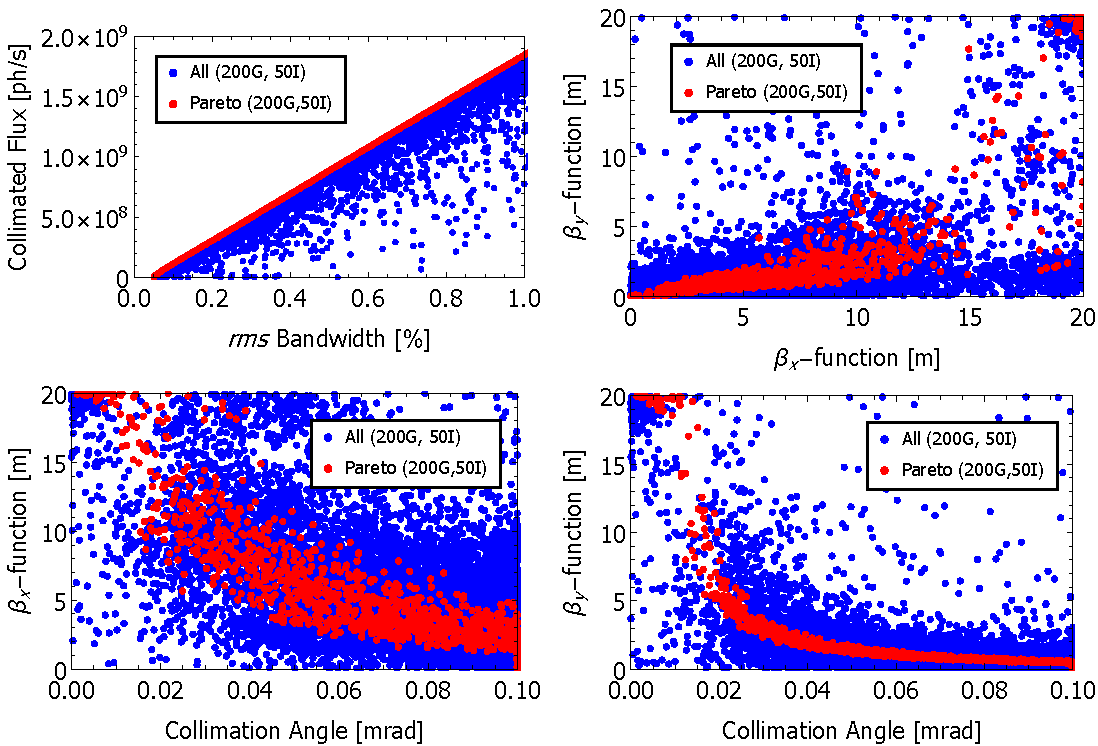
\includegraphics[width=\textwidth]{Figures/Optimisation_and_Characterisation_of_Inverse_Compton_Scattering_Sources/CaseA_GA_Tuning_Curve.pdf}
\caption{Case A genetic algorithm tuning curves (solution and parameter space) produced using 200 generations and 50 individuals, showing the non-dominated Pareto front points (red) and the dominated trial points (blue). Top Left: collimated flux as a function of \textit{rms} bandwidth solution space. Top Right: parameter space plot of the $\beta$-function in the $x$ plane as a function of the $\beta$-function in the $y$ plane at the IP. Bottom Left: parameter space plot of the $\beta_{x}$-function at the IP as a function of the collimation angle. Bottom Right: parameter space plot of the $\beta_{y}$-function at the IP as a function of the collimation angle.}
\label{fig:case_A_GA_tuning_curves}
\end{figure}

In Fig.~\ref{fig:case_A_GA_tuning_curves}, a well defined Pareto-optimal front in the collimated flux--\textit{rms} bandwidth solution space is visible. The individuals in the solution space Pareto-optimal front are clearly non-dominated, with a series of dominated points shown below this front. The resulting Pareto-optimal front is the maximal collimated flux as a function if \textit{rms} bandwidth, and therefore a tuning curve for the case A ICS source. There is also a minimum \textit{rms} bandwidth cut-off at $\sim 0.1$\%, as predicted by Eq.~\ref{eq:bandwidth_limitation_minimum}. A maximum collimated flux of $\sim 1.9\times 10^{9}$~ph/\si{\second} is expected at 1\% \textit{rms} bandwidth.

The $\beta_{x}^{*}$--$\beta_{y}^{*}$ parameter space plot shows that the variables corresponding to the non-dominated solutions do not follow the round beam solution ($\beta_{x}^{*}\neq\beta_{y}^{*}$). Therefore, the round beam solution is sub-optimal and non-round beam simulation is beneficial even when the transverse emittance of the electron beam is round ($\epsilon_{nx}=\epsilon_{ny}=\epsilon_{n}$). Typically, the Pareto-optimal variables favour $\beta_{x}^{*}>\beta_{y}^{*}$ because the crossing angle is imposed in the $x$--$z$ plane; this is the only difference between the two transverse planes. When $\beta_{x}^{*}>10$~\si{\meter} the spread of the optimal $\beta$-functions at the IP becomes large because the parameter space is highly constrained; these correspond to solutions for the narrowest bandwidths. Many dominated individuals exist around the parameter space of the Pareto-optimal individuals in the $\beta_{x}^{*}$--$\beta_{y}^{*}$ parameter space, demonstrating that the parameter space is well explored.

The parameter spaces  of the $\beta$-functions against the collimation angle differ in each plane due to the crossing angle in the $x$--$z$ plane, but both show a characteristic `elbow' shape. The $\beta_{x}$--$\theta_{\mathrm{col}}$ parameter space shows a large stratification in the Pareto-optimal variable positions which shows the objective functions have a weak dependence on this variable, this plot varies largely from the $\beta^{*}$--$\theta_{\mathrm{col}}$ parameter space curve in Fig.~\ref{fig:CaseA_RB_tuning_curve}. In comparison, the $\beta_{y}^{*}$--$\theta_{\mathrm{col}}$ parameter space plot shows far less stratification of the Pareto-optimal front variables and a clearer `elbow' shape of the optimal variables, also present in the parameter space of the RB optimisation in Fig.~\ref{fig:CaseA_RB_tuning_curve}. In both of the $\beta$-function at the IP against collimation angle parameter space plots for case A there appears to be a lack of statistics -- dominated points -- around 0.02~\si{\milli\radian}, the cause of which is unknown though this may be a random occurrence in the optimisation.    